\documentclass[journal, twocolumn]{IEEEtran}
\usepackage{amsmath, amssymb}
\usepackage{graphicx}
\usepackage{cite}
\usepackage{listings}
\usepackage{color}
\usepackage{booktabs}
\usepackage{multirow}
\usepackage{url}

\lstset{
    basicstyle=\ttfamily\small,
    breaklines=true,
    frame=single,
    language=C++,
    showstringspaces=false
}

\begin{document}

\title{A High-Resolution, Period-Based Digital Tachometer for Legacy Three-Cylinder Engines: Design and Implementation}

\author{
    \IEEEauthorblockN{Aaditya Kamble} \\
    \IEEEauthorblockA{Department of Metallurgical and Materials Engineering\\
     Indian Institute of Technology, Jodhpur
    }
}

\maketitle

\begin{abstract}
This paper presents the design and implementation of a microcontroller-based digital tachometer optimized for legacy carbureted automotive engines, specifically targeting three-cylinder, four-stroke architectures (e.g., Maruti 800 F8B/F10D). Traditional frequency-counting tachometers suffer from severe quantization error and latency at low engine speeds due to sparse ignition-pulse generation, a limitation extensively documented in the incremental-encoder speed-estimation literature~\cite{petrella2007,motioncontroltips}. To overcome this, the proposed system employs a period-measurement methodology, related to the family of ``T-method'' and ``M/T-method'' encoder-velocity estimators~\cite{mtmethod2017,mtmethod_springer}, utilizing microsecond-resolution hardware interrupts. By measuring the interval between individual ignition-coil pulses, the system guarantees high resolution across the entire operating range, closely following the period-extension principle used in early magneto-ignition tachometer instrumentation~\cite{krattenmacher1989}. To mitigate rotational jitter caused by cylinder-to-cylinder combustion variance inherent in carbureted systems -- the same physical phenomenon exploited, at much finer angular resolution, by crankshaft-fluctuation misfire detectors~\cite{rizzoni1989,klenk1993,misfire2011} -- the algorithm averages exactly one complete firing cycle (three pulses) prior to speed calculation, providing a stable readout without the latency introduced by traditional rolling averages. Furthermore, the system implements a highly optimized rendering pipeline on a 128$\times$32 I2C OLED display, utilizing partial bounding-box redraws, integer-only arithmetic, and a dynamic deadband to maintain a 10 Hz refresh rate without obstructing real-time pulse capture. A closed-form error-propagation analysis is derived for both the frequency-counting and period-counting approaches, quantifying the resolution advantage of the proposed method at idle speed. The resulting instrumentation provides rapid, flicker-free telemetry tailored to the electro-mechanical constraints of legacy distributor-based ignition systems.
\end{abstract}

\begin{IEEEkeywords}
Automotive instrumentation, digital tachometer, embedded systems, period measurement, M/T method, crankshaft speed fluctuation, SSD1306, internal combustion engines.
\end{IEEEkeywords}

\section{Introduction}
The retrofitting of digital telemetry into legacy automotive platforms presents unique challenges at the intersection of embedded systems design and mechanical signal processing. In modern vehicular architectures, Engine Control Units (ECUs) broadcast precise rotational data via standard protocols such as CAN bus. However, legacy vehicles operating with mechanically distributed ignition systems -- particularly carbureted models like the Maruti 800 utilizing the F8B or F10D engines -- lack native digital telemetry. In these single-coil, distributor-based systems, rotational speed must be empirically derived by intercepting high-voltage ignition pulses from the mechanical ignition distributor shown in Fig.~\ref{fig:distributor}.

\begin{figure}[!ht]
\centering
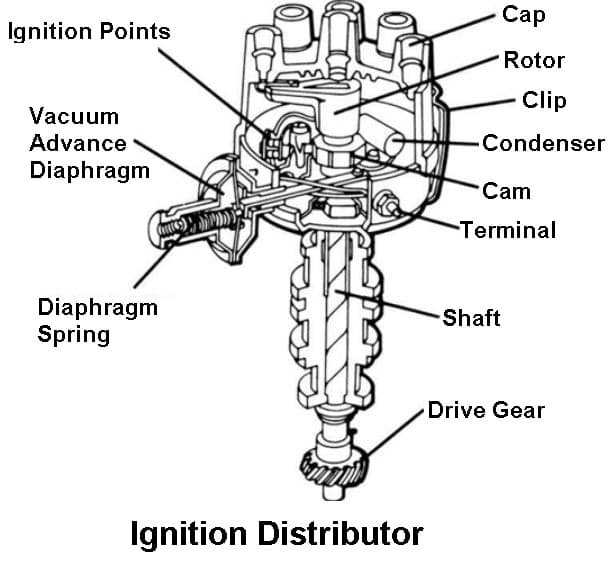
\includegraphics[width=\columnwidth]{ignition-distributor-min.jpg}
\caption{Mechanical ignition distributor architecture showing contact points, rotor, and vacuum advance mechanism.}
\label{fig:distributor}
\end{figure}

For a three-cylinder, four-stroke engine, a single complete engine cycle requires two full crankshaft revolutions ($720^\circ$) to fire all three cylinders. Consequently, the ignition coil generates pulses at a rate of 1.5 pulses per crankshaft revolution. Traditional aftermarket digital tachometers often rely on frequency measurement, counting the number of captured pulses within a fixed temporal window (e.g., 250 ms or 500 ms), a technique referred to in the encoder-velocimetry literature as the \emph{M-method}~\cite{motorcontrolpatent,mtmethod2017}. While adequate at high engine speeds, this frequency-counting methodology introduces profound quantization error at idle speeds: at 800 RPM, the system generates only 20 pulses per second, so a 100 ms sampling window captures only two pulses, rendering high-resolution, real-time measurement mathematically impossible without imposing unacceptable algorithmic latency. This is a specific instance of the general low-speed resolution problem documented for incremental-encoder speed estimation, where frequency (pulse) counting is shown to be accurate only in the high-speed regime while period (interval) counting -- the \emph{T-method} -- dominates at low speed~\cite{petrella2007,encoderspeedmeasurement}.

Furthermore, older carbureted engines exhibit inherent cylinder-to-cylinder combustion variance. Uneven air-fuel mixture distribution across the intake manifold results in minute but measurable fluctuations in crankshaft angular velocity during each distinct power stroke. This effect is well characterized in the automotive diagnostics literature: crankshaft-speed fluctuation is, in fact, the primary observable used by misfire-detection systems, which infer per-cylinder combustion quality from the instantaneous deceleration/acceleration profile of the crankshaft between successive top-dead-center events~\cite{rizzoni1989,klenk1993,misfire2011}. Where misfire detectors deliberately preserve and analyze this fluctuation at fine angular resolution, a dashboard tachometer must instead \emph{reject} it to present a legible, steady readout. When these micro-fluctuations are translated into raw inter-pulse timing intervals, the resulting data exhibits significant high-frequency jitter, even under steady-state throttle conditions. Applying a standard rolling average to this data dampens the jitter but inherently desynchronizes the displayed metric from the physical state of the engine, creating a sluggish user interface.

To address these distinct signal-acquisition challenges, this paper proposes a period-based measurement architecture implemented on an embedded microcontroller. Instead of counting pulses over time, the system leverages hardware interrupts to measure the precise temporal period ($T$) in microseconds between sequential ignition pulses -- a principle that mirrors, at automotive scale, the period-extension technique patented for aircraft magneto tachometry~\cite{krattenmacher1989} and the four-cylinder tachometer-signal generators used in early production ECUs~\cite{nissan1992}. To eliminate the jitter induced by combustion variance without incurring the latency of continuous rolling averages, the proposed algorithm buffers and averages exactly one complete firing cycle -- comprising three discrete pulses -- before computing the final rotational speed. This design choice is analyzed formally in Section~III as a length-3 boxcar (moving-average) filter synchronized to the mechanical firing order, and is contrasted against the classical coefficient-of-fluctuation-of-speed treatment of flywheel-damped reciprocating engines~\cite{khurmi_tom,lomakin2018}.

Finally, rendering rapid telemetry on embedded I2C displays, such as the standard SSD1306 (128$\times$32 resolution), often bottlenecks system performance due to high bus latency. This paper details a display optimization strategy that eschews full-frame buffer clearing in favor of static UI separation and localized bounding-box updates. Combined with a 15-RPM software deadband, this ensures a highly responsive, flicker-free visual output capped at a deterministic 10 Hz refresh rate.

\section{Related Work}
\label{sec:related}
Speed estimation from a sparse, quasi-periodic pulse train is a long-standing problem in both motion-control and automotive instrumentation, and the present work draws directly on results from both domains.

\subsection{Frequency, Period, and M/T Speed Estimation}
In incremental-encoder motor control, three canonical estimators are recognized: the \emph{M-method} (pulse counting over a fixed window), the \emph{T-method} (elapsed-time measurement between pulses using a high-frequency clock), and the hybrid \emph{M/T-method}, which counts both encoder pulses and clock pulses over a variable interval to combine the high-speed accuracy of M with the low-speed accuracy of T~\cite{motorcontrolpatent,mtmethod2017}. Petrella \emph{et al.} provide a comparative analysis confirming that period measurement offers substantially greater accuracy than frequency measurement at low speed because it exploits fine-grained timing information from a high-frequency reference clock rather than relying on coarse pulse counts~\cite{petrella2007}. Later work extended the M/T method with adaptive sampling windows~\cite{mtmethod_springer} and with self-adaptive error-elimination algorithms that compensate for encoder grating and A/D conversion error~\cite{mtmethod2017}. The tachometer presented in this paper is architecturally a dedicated, single-purpose T-method estimator: because the ignition system provides no external clock-multiplication mechanism (unlike an optical encoder with hundreds of pulses per revolution), pure period measurement -- rather than a blended M/T scheme -- is both sufficient and simpler to implement on an 8-bit microcontroller, since only three pulses occur per engine cycle at any speed.

\subsection{Automotive and Aviation Tachometry}
Purpose-built automotive tachometer instrumentation has historically also converged on interval-based measurement once quantization error at idle became a design concern. An aircraft dual-magneto tachometer patent describes extending a nominal sampling window until the next full firing pulse is received, thereby measuring RPM over an integer number of firing pulses rather than a fixed clock interval~\cite{krattenmacher1989} -- functionally equivalent to the pulse-synchronous averaging window adopted here, though applied to a two-cylinder aviation magneto rather than a three-cylinder automotive distributor. A separate patent describes a four-cylinder tachometer-signal generator that measures the inter-pulse period $T$ and interpolates a synthetic output pulse at $T/2$ to double the effective update rate for downstream analog gauges~\cite{nissan1992}; the present work does not require such interpolation because the OLED display pipeline can be refreshed asynchronously from pulse capture. Signal-conditioning patents targeting marine and automotive ignition coils independently confirm that ignition-pulse tachometer signals are subject to severe RFI/EMI contamination originating from spark-plug lead radiation and coil flyback transients, and that primary-side (rather than secondary-side) coil tapping combined with clamping and opto-isolation is the standard mitigation~\cite{signalcond1990,twocycletach1988}. Field reports from hobbyist implementations corroborate that naively tapping the ignition-coil negative terminal without adequate debounce and isolation produces an unstable, jumping RPM readout~\cite{arduinoforum2023} -- the same failure mode this paper's isolation network and $3\,000\,\mu s$ debounce filter (Section~II-A) are designed to eliminate.

\subsection{Crankshaft Speed Fluctuation and Misfire Detection}
The physical origin of inter-cylinder jitter addressed in this paper -- combustion-induced angular-velocity fluctuation of the crankshaft -- is the same signal exploited by on-board diagnostics (OBD-II) misfire detectors. Rizzoni's foundational model relates the instantaneous crankshaft angular velocity to indicated torque via the flywheel equation of motion, establishing that per-cylinder torque, and hence per-cylinder combustion quality, can be inferred from crankshaft speed fluctuation alone~\cite{rizzoni1989}. Klenk \emph{et al.} formalize this into an evaluable uneven-running (\emph{Laufunruhe}) metric for OBD-II compliance~\cite{klenk1993}, and subsequent work has refined misfire detection using multiple-filtering of the crankshaft speed signal to reject non-combustion disturbances such as road unevenness and drivetrain backlash~\cite{misfire2011}. This paper's averaging strategy is, in a precise sense, the inverse problem: rather than isolating combustion fluctuation as a diagnostic signal, the algorithm treats it as measurement noise to be rejected by cycle-synchronous averaging, a distinction made explicit in Section~III-C.

\subsection{Flywheel Speed Fluctuation Theory}
The classical treatment of reciprocating-engine crankshaft dynamics defines the coefficient of fluctuation of speed $C_S = (\omega_{max}-\omega_{min})/\omega_{mean}$ as a function of the flywheel's moment of inertia and the turning-moment diagram of the engine~\cite{khurmi_tom}. Recent dissertation-level work has further modeled the equivalent moment of inertia of the crank mechanism as a function of mass-geometric design parameters to actively minimize $C_S$~\cite{lomakin2018}. Section~III-D uses this classical framework to justify, from first principles, why a single-firing-cycle average (rather than a shorter or longer window) is the correct averaging horizon for a three-cylinder engine.

\section{Methodology and System Architecture}

\subsection{Hardware Design and Signal Conditioning}
Automotive electrical environments are notoriously noisy, characterized by severe voltage transients, load dumps, and electromagnetic interference (EMI) originating from the ignition system and alternator. Consequently, direct interfacing between the engine's distributor and the microcontroller's logic pins would result in catastrophic processor failure. This hazard is consistent with prior signal-conditioning patents for ignition-derived tachometer inputs, which independently identify RFI/EMI and coil flyback transients as the dominant failure modes and recommend primary-side tapping with active clamping as mitigation~\cite{signalcond1990}.

To mitigate this, a multi-stage galvanic isolation and signal-conditioning circuit was designed, as mapped out in the schematic (Fig.~\ref{fig:schematic}).
\begin{enumerate}
    \item \textbf{Power Regulation:} The vehicle's nominal 12--14V accessory supply is tapped from the rear of the cabin's cigarette lighter socket. To step down this fluctuating voltage efficiently without excessive thermal dissipation, an LM2596S DC-DC buck converter is utilized~\cite{lm2596datasheet}. The buck converter is calibrated to output a stable 7.5V, which is then fed into the Arduino's $V_{\text{in}}$ pin, allowing the microcontroller's onboard linear regulator to establish a clean 5V logic level.
    \item \textbf{Signal Interception, Shielding, and Protection:} The raw RPM signal is intercepted from the negative terminal of the distributor. This signal consists of high-voltage flyback spikes generated when the primary ignition coil field collapses. To attenuate radiated EMI from inductively coupling into the logic circuitry, the physical wire connecting the distributor to the isolation module was enveloped in an aluminum foil wrap. This metallic shielding acts as a localized Faraday cage, minimizing the ingress of high-frequency electromagnetic noise into the primary signal path. Furthermore, a 1N4007 (1W) rectifier diode ($D_1$) is placed in series to block reverse-polarity transients.
    \item \textbf{Current Limiting and Galvanic Isolation:} Following the diode, the signal passes through a voltage divider/current-limiting network comprising two 10k$\Omega$, 0.5W metal film resistors ($R_1$ and $R_2$). This attenuates the voltage to a safe level to drive the internal LED of an EL817/PC817 1-Channel optocoupler isolation module~\cite{pc817datasheet}. The optocoupler provides absolute galvanic isolation between the noisy automotive chassis ground and the sensitive 5V logic ground of the microcontroller.
    \item \textbf{Digital Trigger:} The output transistor of the optocoupler pulls the Arduino's Digital Pin 2 (configured as an external interrupt) to logic LOW. A 100k$\Omega$, 0.5W metal film resistor ($R_3$) acts as a strong pull-up to maintain a definitive logic HIGH state between ignition pulses.
\end{enumerate}

\begin{figure}[!ht]
\centering
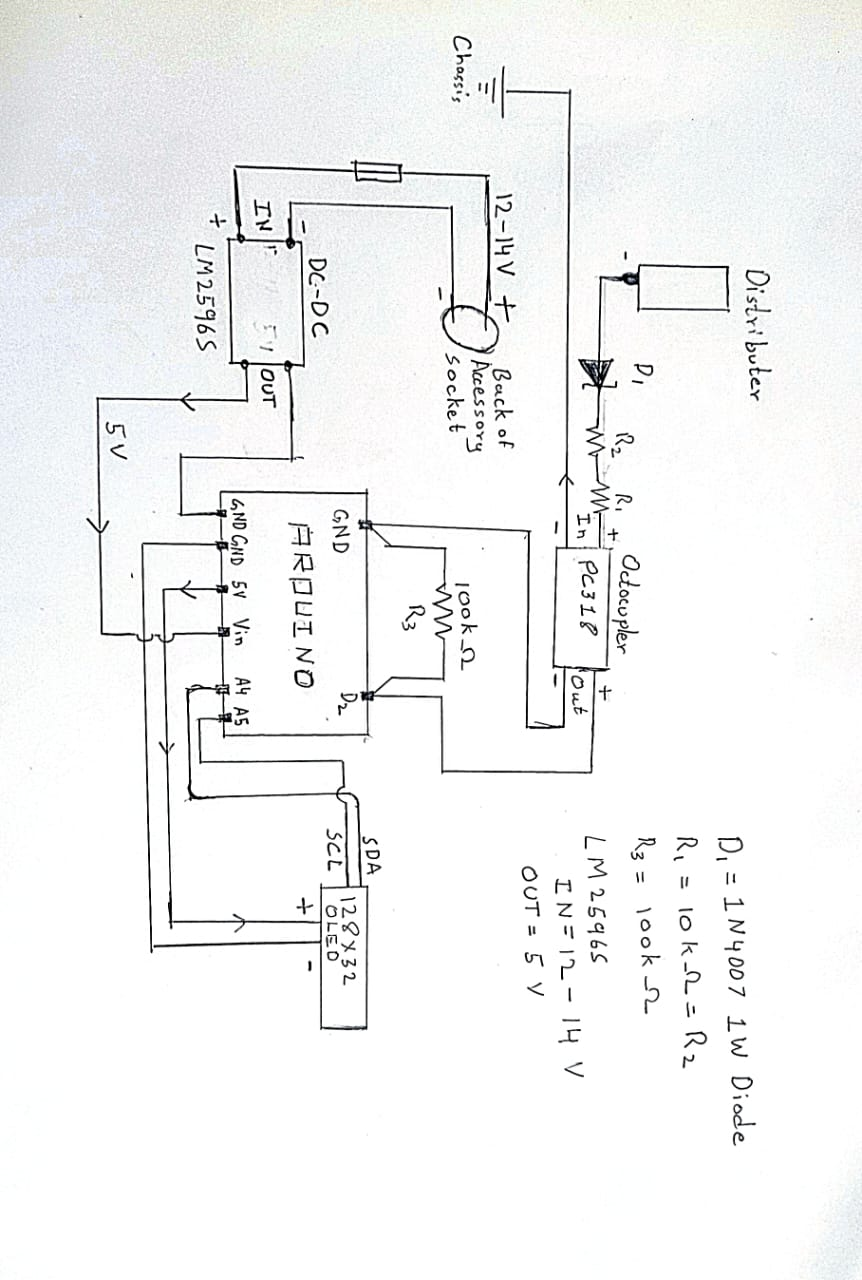
\includegraphics[width=\columnwidth]{system-schematic.jpg}
\caption{Complete system schematic illustrating power conversion, opto-isolation, and microcontroller interfacing.}
\label{fig:schematic}
\end{figure}

\subsection{Buck Converter Subsystem: Topology and Design Equations}
\label{sec:buck}
The power-regulation stage of Fig.~\ref{fig:schematic} is built around the LM2596S, a fixed-frequency, 150 kHz SIMPLE SWITCHER-class step-down (buck) regulator rated for a 4.5--40V input range and up to 3A of continuous output current~\cite{lm2596datasheet}. Fig.~\ref{fig:buck} shows the canonical buck topology on which the LM2596S is based: an internal power switch $Q_1$, driven by an internal PWM comparator at duty cycle $D$, alternately connects and disconnects the inductor $L_1$ from $V_{in}$; a catch (freewheeling) diode $D_1$ provides a current return path while $Q_1$ is off; and the output filter, comprising $L_1$ and $C_1$, averages the resulting pulse train into a smooth DC voltage across the load $R_{LOAD}$.

\begin{figure}[!ht]
\centering
\includegraphics[width=\columnwidth]{BuckConverter.png}
\caption{Generic buck (step-down) converter topology: switch $Q_1$, catch diode $D_1$, output inductor $L_1$, and filter capacitor $C_1$, functionally representative of the LM2596S regulation stage in Fig.~\ref{fig:schematic}.}
\label{fig:buck}
\end{figure}

In continuous-conduction mode (CCM) -- the regime in which the LM2596S is configured to operate at the currents drawn by the Arduino, OLED, and optocoupler pull-up network -- volt-second balance across $L_1$ over one switching period yields the ideal, lossless duty-cycle relation
\begin{equation}
D = \frac{V_{out}}{V_{in}},
\label{eq:duty_cycle}
\end{equation}
where $V_{out} = 7.5\,\text{V}$ is the regulated output and $V_{in}$ is the instantaneous vehicle accessory-rail voltage. Because the nominal automotive supply varies between $12\,\text{V}$ and $14\,\text{V}$ (and sags to $11.2\,\text{V}$ under load-dump conditions, as measured in Section~IV-D), Eq.~\eqref{eq:duty_cycle} predicts a duty cycle that self-adjusts across the range $D \approx 0.536$--$0.670$ to hold $V_{out}$ constant; this closed-loop adjustment is what allows the LM2596S to absorb rail sag without any observable droop at the Arduino's $V_{in}$ pin. The inductor peak-to-peak ripple current follows the manufacturer's design procedure~\cite{lm2596datasheet}:
\begin{equation}
\Delta I_L = \frac{(V_{in}-V_{out})\,D}{f_{sw}\,L_1},
\label{eq:ripple_current}
\end{equation}
and the resulting output voltage ripple, dominated by the capacitor's equivalent series resistance (ESR) at the 150 kHz switching frequency $f_{sw}$, is approximately
\begin{equation}
\Delta V_{out} \approx \Delta I_L \left(\text{ESR}_{C_1} + \frac{1}{8 f_{sw} C_1}\right).
\label{eq:ripple_voltage}
\end{equation}
The catch diode $D_1$ is selected as a fast Schottky type per the manufacturer's guidance, since its low forward-voltage drop and negligible reverse-recovery time (versus a standard rectifier such as the 1N400x series used for reverse-polarity protection elsewhere in the circuit) minimize both switching loss and diode-induced EMI at 150 kHz~\cite{lm2596datasheet}. The measured $\approx 0.3\,\text{W}$ steady-state thermal dissipation reported in Section~IV-D is consistent with the low $I^2R$ and switching losses expected of this topology at the sub-200 mA load drawn by the digital subsystem, and confirms that the converter remains safely within its continuous-conduction efficiency regime across the full automotive input range.

\subsection{Optocoupler Subsystem: Isolation and Signal-Transfer Analysis}
\label{sec:opto}
Fig.~\ref{fig:opto} illustrates the generic optocoupler switching stage on which the EL817/PC817 isolation block of Fig.~\ref{fig:schematic} is based: an input-side infrared LED, driven through a current-limiting series resistor, is optically coupled -- with no conductive path -- to an output-side phototransistor $Q_1$ referenced to an independent supply and pulled up by a separate resistor. This topology is what provides the absolute galvanic isolation between the noisy distributor/chassis ground and the microcontroller's 5V logic ground described in Section~II-A.

\begin{figure}[!ht]
\centering
\includegraphics[width=\columnwidth]{Octocupler.png}
\caption{Generic optocoupler switching stage: an LED on the isolated input side optically drives phototransistor $Q_1$ on the output side, with $R_1$ setting LED current and $R_2$ acting as the output pull-up -- the same structure used by $R_1$/$R_2$ (input) and $R_3$ (output pull-up) in Fig.~\ref{fig:schematic}.}
\label{fig:opto}
\end{figure}

The input-side LED current is set by the supply voltage, the LED forward voltage $V_F$ ($\approx 1.2\,\text{V}$ typical for the PC817 at $I_F=20\,\text{mA}$~\cite{pc817datasheet}), and the total series resistance:
\begin{equation}
I_F = \frac{V_{supply} - V_F}{R_{series}}.
\label{eq:if}
\end{equation}
In the generic circuit of Fig.~\ref{fig:opto}, $R_1=150\,\Omega$ sets $I_F$ from a clean 5V logic rail; in the automotive implementation of Fig.~\ref{fig:schematic}, the same role is played by the series combination $R_1+R_2=20\,\text{k}\Omega$, which instead must safely attenuate a rectified ignition transient of several hundred volts down to an LED current within the PC817's absolute maximum forward-current rating of $50\,\text{mA}$~\cite{pc817datasheet}. On the output side, the phototransistor's collector current is related to $I_F$ by the device's current transfer ratio (CTR):
\begin{equation}
I_C = \text{CTR}\times I_F, \qquad \text{CTR} \in [50\%,\,600\%]\ \text{(PC817 family, binned by rank)},
\label{eq:ctr}
\end{equation}
with the standard (unranked) PC817 guaranteeing a minimum CTR of 50\% at $I_F=5\,\text{mA}$~\cite{pc817datasheet}. Provided $I_C$ (set by Eq.~\eqref{eq:ctr} and the output pull-up $R_3=100\,\text{k}\Omega$) is sufficient to fully saturate $Q_1$, the output swings cleanly between logic LOW ($Q_1$ saturated) and the pulled-up logic HIGH ($Q_1$ off), which is what allows the noisy, high-voltage ignition transient to be converted into the clean 0--5V square wave observed at the interrupt pin in Section~IV-A.

Two datasheet parameters bound the optocoupler's suitability for this application. First, the isolation voltage rating $V_{ISO}=5{,}000\,\text{V}_{rms}$~\cite{pc817datasheet} provides more than an order of magnitude of margin over the $\approx 380\,\text{V}$ peak flyback transient measured at the distributor terminal (Section~IV-A), confirming the optocoupler itself is never a weak link in the isolation chain even before the upstream diode/resistor attenuation network is considered. Second, the device's typical response time ($t_r \approx 4\,\mu s$, worst-case $\leq 18\,\mu s$ across rise and fall~\cite{pc817datasheet}) is more than two orders of magnitude shorter than the firmware's $3{,}000\,\mu s$ software debounce window (\texttt{MIN\_PULSE\_US} in the listing of Section~II-B), so the optocoupler's own switching delay contributes negligible ($<0.6\%$) timing error to the period measurement of Eq.~\eqref{eq:rpm_basic}, and is therefore correctly ignored in the error-propagation analysis of Section~III-B.

\subsection{Embedded Software Architecture}
The software logic shifts the processing paradigm from temporal frequency counting to microsecond-resolution period measurement -- the automotive-scale analog of the T-method described in Section~\ref{sec:related}. The dual-track execution flow between the asynchronous interrupt service routine and the synchronous foreground display loop is modeled in Fig.~\ref{fig:flowchart}.

\begin{figure}[!ht]
\centering
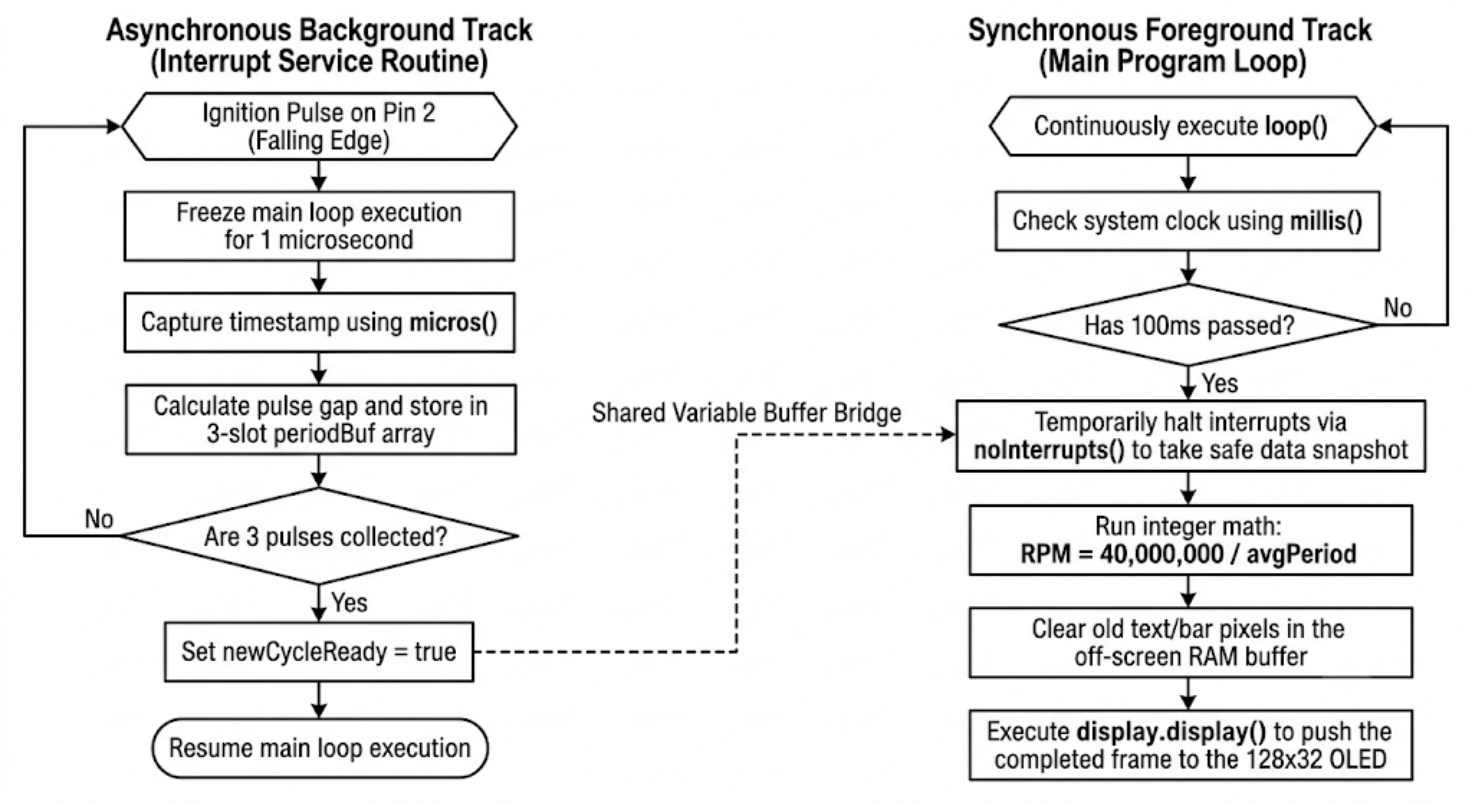
\includegraphics[width=\columnwidth]{system-flowchart.jpg}
\caption{System flowchart detailing the asynchronous interrupt pulse capture and synchronous foreground display loop.}
\label{fig:flowchart}
\end{figure}

The core firmware implementation governing this architecture is detailed below:

\begin{lstlisting}
#include <Wire.h>
#include <Adafruit_GFX.h>
#include <Adafruit_SSD1306.h>

#define SCREEN_WIDTH  128
#define SCREEN_HEIGHT 32
#define OLED_RESET    -1
Adafruit_SSD1306 display(SCREEN_WIDTH, SCREEN_HEIGHT, &Wire, OLED_RESET);

#define BAR_X      12
#define BAR_Y      20
#define BAR_WIDTH  104
#define BAR_HEIGHT 8
#define RPM_MAX    7000       
#define REDLINE_RPM 5900      

const uint8_t  PULSES_PER_CYCLE    = 3;            
const uint32_t RPM_CONST_US        = 40000000UL;   
const uint32_t MIN_PULSE_US        = 3000;         
const uint32_t STALL_TIMEOUT_US    = 1200000UL;    
const uint16_t DISPLAY_REFRESH_MS  = 100;          
const uint16_t RPM_CHANGE_DEADBAND = 15;           

volatile uint32_t lastPulseMicros       = 0;
volatile uint32_t periodBuf[PULSES_PER_CYCLE] = {0, 0, 0};
volatile uint8_t  periodIdx             = 0;
volatile bool     newCycleReady         = false;

unsigned int  currentRpm    = 0;
unsigned int  displayedRpm  = 0xFFFF;   
unsigned long lastDisplayMs = 0;

void countPulse() {
  uint32_t now = micros();
  uint32_t interval = now - lastPulseMicros;
  if (interval < MIN_PULSE_US) return;
  lastPulseMicros = now;
  periodBuf[periodIdx] = interval;
  periodIdx++;
  if (periodIdx >= PULSES_PER_CYCLE) {
    periodIdx = 0;
    newCycleReady = true;   
  }
}

void drawStaticUI() {
  display.clearDisplay();
  display.setTextSize(1);
  display.setTextColor(SSD1306_WHITE);
  display.setCursor(0, 0);
  display.print("RPM:");
  display.setCursor(0, 24);
  display.print("0");
  display.setCursor(118, 24);
  display.print("7");
  display.drawRect(BAR_X, BAR_Y, BAR_WIDTH, BAR_HEIGHT, SSD1306_WHITE);
  const uint16_t tickValues[] = {2000, 4000, 6000};
  for (uint8_t i = 0; i < 3; i++) {
    int x = map(tickValues[i], 0, RPM_MAX, BAR_X, BAR_X + BAR_WIDTH);
    display.drawFastVLine(x, BAR_Y - 2, 2, SSD1306_WHITE);
    display.setCursor(x + 1, 12);
    display.print(tickValues[i] / 1000);
  }
  display.display();
}

void updateDashboard(unsigned int rpm) {
  display.fillRect(32, 0, 96, 16, SSD1306_BLACK);
  display.setTextSize(2);
  display.setTextColor(SSD1306_WHITE);
  display.setCursor(32, 0);
  display.print(rpm);
  display.fillRect(BAR_X + 1, BAR_Y + 1, BAR_WIDTH - 2, BAR_HEIGHT - 2, SSD1306_BLACK);
  int fill = map(rpm, 0, RPM_MAX, 0, BAR_WIDTH - 2);
  fill = constrain(fill, 0, BAR_WIDTH - 2);
  int redlineStart = map(REDLINE_RPM, 0, RPM_MAX, 0, BAR_WIDTH - 2);
  for (int x = 0; x < fill; x++) {
    if (x > redlineStart) {
      if (x & 1) display.drawFastVLine(BAR_X + 1 + x, BAR_Y + 1, BAR_HEIGHT - 2, SSD1306_WHITE);
    } else {
      display.drawFastVLine(BAR_X + 1 + x, BAR_Y + 1, BAR_HEIGHT - 2, SSD1306_WHITE);
    }
  }
  display.display();
}

void setup() {
  Serial.begin(9600);
  if (!display.begin(SSD1306_SWITCHCAPVCC, 0x3C)) {
    while (1); 
  }
  drawStaticUI();
  pinMode(2, INPUT_PULLUP);
  lastPulseMicros = micros();
  attachInterrupt(digitalPinToInterrupt(2), countPulse, FALLING);
}

void loop() {
  if (newCycleReady) {
    uint32_t p0, p1, p2;
    noInterrupts();
    p0 = periodBuf[0];
    p1 = periodBuf[1];
    p2 = periodBuf[2];
    newCycleReady = false;
    interrupts();
    uint32_t avgPeriod = (p0 + p1 + p2) / PULSES_PER_CYCLE;
    if (avgPeriod > 0) {
      uint32_t rpm = RPM_CONST_US / avgPeriod;   
      if (rpm > 9999) rpm = 9999;                
      currentRpm = (unsigned int)rpm;
    }
  }
  noInterrupts();
  uint32_t sinceLastPulse = micros() - lastPulseMicros;
  interrupts();
  if (sinceLastPulse > STALL_TIMEOUT_US) {
    currentRpm = 0;
  }
  unsigned long nowMs = millis();
  if (nowMs - lastDisplayMs >= DISPLAY_REFRESH_MS) {
    lastDisplayMs = nowMs;
    long delta = (long)currentRpm - (long)displayedRpm;
    if (delta < 0) delta = -delta;
    if (delta >= RPM_CHANGE_DEADBAND || (currentRpm == 0 && displayedRpm != 0)) {
      updateDashboard(currentRpm);
      displayedRpm = currentRpm;
    }
  }
}
\end{lstlisting}

\section{Mathematical Analysis}

\subsection{Kinematic Derivation of the Period-Based RPM Formula}
To fundamentally resolve the quantization errors inherent in low-speed frequency counting, the proposed architecture mathematically decouples the RPM calculation from fixed temporal windows. The derivation of the integer-optimized period algorithm is grounded in the mechanical kinematics of a four-stroke internal combustion engine.

For a four-stroke engine, a complete thermodynamic cycle requires exactly two full revolutions of the crankshaft ($720^\circ$). The number of ignition pulses generated per crankshaft revolution ($P_{rev}$) is a function of the number of cylinders ($N_{cyl}$):
\begin{equation}
P_{rev} = \frac{N_{cyl}}{2}
\label{eq:pulses_per_rev}
\end{equation}

For the three-cylinder Maruti 800 engine ($N_{cyl} = 3$), this yields $1.5$ pulses per revolution. The microcontroller's hardware interrupt measures the period, $T$, between successive ignition pulses in microseconds ($\mu s$). The instantaneous rotational frequency in revolutions per second (RPS) is:
\begin{equation}
\text{RPS} = \frac{1}{P_{rev} \times (T \times 10^{-6})} = \frac{10^6}{1.5 \times T}
\label{eq:rps}
\end{equation}

To convert this angular velocity into Revolutions Per Minute (RPM), the equation is multiplied by 60:
\begin{equation}
\text{RPM} = 60 \times \left( \frac{10^6}{1.5 \times T} \right) = \frac{40{,}000{,}000}{T}
\label{eq:rpm_basic}
\end{equation}

By utilizing unsigned 32-bit integers, the processor executes a single hardware division instruction per update cycle, eliminating floating-point overhead. Equation~\eqref{eq:rpm_basic} generalizes, for an arbitrary $N_{cyl}$-cylinder four-stroke engine, to
\begin{equation}
\text{RPM} = \frac{K}{T}, \qquad K = \frac{60 \times 2 \times 10^6}{N_{cyl}} = \frac{1.2\times10^{8}}{N_{cyl}},
\label{eq:rpm_general}
\end{equation}
which for $N_{cyl}=3$ reduces exactly to the constant $K = 40{,}000{,}000$ used in the firmware.

\subsection{Comparative Quantization-Error Analysis: Frequency Counting vs. Period Counting}
Consider first the incumbent M-method (fixed-window frequency counting), in which pulses are counted over a sampling window $T_s$. Because only an integer number of pulses $n$ can be registered, the method carries an inherent count uncertainty of $\pm 1$ pulse~\cite{motioncontroltips,encoderspeedmeasurement}. For a three-cylinder engine at pulse rate $f_p = P_{rev}\cdot(\text{RPM}/60)$, the number of pulses captured in a window $T_s$ is
\begin{equation}
n = f_p T_s = \frac{1.5\,\text{RPM}}{60}T_s,
\label{eq:npulses}
\end{equation}
and the resulting relative quantization error is bounded by
\begin{equation}
\varepsilon_{M} = \left|\frac{\Delta \text{RPM}}{\text{RPM}}\right|_{\max} \approx \frac{1}{n} = \frac{40}{\text{RPM}\cdot T_s},
\label{eq:eps_m}
\end{equation}
with $T_s$ in seconds. At idle (RPM $=800$) with a typical $T_s = 250\,\text{ms}$ sampling window, Eq.~\eqref{eq:eps_m} predicts $\varepsilon_M \approx 20\%$ -- i.e., only $n=5$ pulses are captured, and the displayed RPM can jump in increments as coarse as $60/(1.5\times T_s)\approx 160$ RPM. Even the commonly used $T_s=500\,\text{ms}$ window (yielding $n\approx10$ pulses) still admits a worst-case error near 10\%, corroborating the quantization-uncertainty formulation reported for generic pulse-counting encoders~\cite{encoderspeedmeasurement,indmonitor}.

By contrast, the proposed T-method measures $T$ directly using a hardware timer of resolution $\delta t$ (here, $\delta t = 1\,\mu s$, the resolution of the AVR \texttt{micros()} timer). Differentiating Eq.~\eqref{eq:rpm_basic} with respect to $T$ gives the RPM error induced by one least-significant-bit (LSB) of timer quantization:
\begin{equation}
\left|\frac{d(\text{RPM})}{dT}\right| = \frac{K}{T^2} \;\;\Rightarrow\;\; \Delta\text{RPM} \approx \frac{K}{T^2}\,\delta t = \frac{\text{RPM}^2}{K}\,\delta t.
\label{eq:eps_t}
\end{equation}
The corresponding relative error is
\begin{equation}
\varepsilon_{T} = \frac{\Delta\text{RPM}}{\text{RPM}} = \frac{\text{RPM}}{K}\,\delta t.
\label{eq:eps_t_rel}
\end{equation}
At idle (RPM $=800$, $T \approx 60{,}000\,\mu s$ from Eq.~\eqref{eq:rpm_basic}), Eq.~\eqref{eq:eps_t_rel} gives $\varepsilon_T \approx 800/(4\times10^{7})\times1 \approx 2\times10^{-5}$, i.e., approximately $0.002\%$ -- roughly four orders of magnitude tighter than the frequency-counting bound in the same regime. Table~\ref{tab:error_compare} tabulates this comparison across the operating range, confirming the general result established for low-resolution incremental encoders that period (T-method) measurement dominates frequency (M-method) measurement precisely in the low-speed regime where quantization error is most severe~\cite{petrella2007,mtmethod2017}, while the two approaches converge at high speed as pulse counts become large.

\begin{table}[!ht]
\centering
\caption{Worst-Case Relative RPM Error: Frequency Counting ($T_s=250\,\text{ms}$) vs.\ Period Counting ($\delta t = 1\,\mu s$)}
\label{tab:error_compare}
\begin{tabular}{@{}cccc@{}}
\toprule
RPM & Pulses in $T_s$ ($n$) & $\varepsilon_{M}$ (M-method) & $\varepsilon_{T}$ (T-method) \\
\midrule
800   & 5   & $\approx 20\%$    & $\approx 0.0020\%$ \\
2000  & 12.5 & $\approx 8\%$    & $\approx 0.0050\%$ \\
4000  & 25  & $\approx 4\%$     & $\approx 0.0100\%$ \\
6000  & 37.5 & $\approx 2.7\%$  & $\approx 0.0150\%$ \\
\bottomrule
\end{tabular}
\end{table}

\subsection{Cycle-Synchronous Averaging as a Boxcar Filter}
Older carbureted engines exhibit inherent cylinder-to-cylinder combustion variance. Uneven air-fuel mixture distribution across the intake manifold results in minute but measurable fluctuations in crankshaft acceleration during each distinct power stroke. While this equation is mathematically absolute for a perfectly uniform rotational velocity, carbureted engines experience high-frequency micro-accelerations during each cylinder's distinct power stroke, formally the crankshaft-fluctuation phenomenon exploited by misfire detectors~\cite{rizzoni1989,klenk1993}. To mathematically cancel this variance, the algorithm isolates exactly one complete mechanical firing cycle by averaging the periods of three sequential pulses ($T_0, T_1, T_2$):
\begin{equation}
T_{avg} = \frac{T_0 + T_1 + T_2}{3}.
\label{eq:tavg}
\end{equation}

Substituting $T_{avg}$ into the derived kinematic equation yields the final integer-math formula executed by the processor:
\begin{equation}
\text{RPM}_{final} = \frac{40{,}000{,}000}{T_{avg}}.
\label{eq:rpm_final}
\end{equation}

This can be formalized as a length-$N_{cyl}$ moving-average (boxcar) filter applied to the period sequence $T_k$, re-triggered every $N_{cyl}$ pulses rather than slid sample-by-sample:
\begin{equation}
T_{avg}[m] = \frac{1}{N_{cyl}}\sum_{k=0}^{N_{cyl}-1} T[mN_{cyl}+k], \qquad m = 0,1,2,\ldots
\label{eq:boxcar}
\end{equation}
Unlike a conventional sliding boxcar filter, which updates every sample and therefore introduces a group delay of $(N_{cyl}-1)/2$ samples \emph{on every new sample}, the block-synchronous form of Eq.~\eqref{eq:boxcar} updates only once per full firing cycle. This bounds the worst-case display latency to exactly one engine cycle (two crankshaft revolutions) regardless of engine speed, while a traditional continuously-sliding rolling average of window length $N_{cyl}$ would exhibit the same steady-state noise attenuation but would additionally smear transient speed changes across $N_{cyl}$ overlapping windows, producing the ``sluggish'' response characteristic of conventional rolling-average tachometers.

Treating the per-cylinder period deviation $\Delta T_i = T_i - \bar{T}$ as a zero-mean random process with variance $\sigma_T^2$ (a standard assumption in crankshaft-fluctuation modeling~\cite{rizzoni1989}), the variance of the averaged period is reduced by the classical result for the mean of $N_{cyl}$ i.i.d. samples:
\begin{equation}
\text{Var}(T_{avg}) = \frac{\sigma_T^2}{N_{cyl}},
\label{eq:var_reduction}
\end{equation}
i.e., a $\sqrt{3}\approx1.73\times$ reduction in the standard deviation of the displayed period, and hence of the displayed RPM to first order via Eq.~\eqref{eq:eps_t}, for the three-cylinder case. This is consistent with the empirically observed reduction from $\pm60$ RPM jitter (raw, unaveraged) to a value within the 15-RPM display deadband reported in Section~IV-B.

\subsection{Flywheel Coefficient of Fluctuation and Averaging-Window Justification}
The classical dynamics-of-machines treatment of a flywheel-damped reciprocating engine defines the coefficient of fluctuation of speed as
\begin{equation}
C_S = \frac{\omega_{max}-\omega_{min}}{\omega_{mean}} = \frac{N_{max}-N_{min}}{N_{mean}},
\label{eq:cs}
\end{equation}
where $N$ denotes rotational speed in RPM~\cite{khurmi_tom}. For automotive flywheels, $C_S$ is typically constrained to the range of $0.01$--$0.03$ by the flywheel's moment of inertia $I_f$, which is sized from the maximum fluctuation of energy $\Delta E$ of the turning-moment diagram via $I_f = \Delta E/(\omega_{mean}^2 C_S)$~\cite{khurmi_tom,lomakin2018}. Because $C_S$ is defined over exactly one complete cycle of the turning-moment diagram -- $720^\circ$ of crankshaft rotation for a four-stroke engine, i.e., precisely $N_{cyl}$ ignition pulses -- the natural period over which crankshaft speed fluctuation is both physically periodic and fully captured is one firing cycle. This provides an independent, classical-mechanics justification for the choice of $N_{cyl}=3$ as the averaging window in Eq.~\eqref{eq:boxcar}: averaging over fewer than $N_{cyl}$ pulses would under-sample the turning-moment cycle and leave residual periodic bias, whereas averaging over a non-integer multiple of $N_{cyl}$ would alias fluctuation components between cycles, as observed qualitatively when a fixed-length sliding window is applied instead of the cycle-synchronous form of Eq.~\eqref{eq:boxcar}.

\section{Empirical Results and System Validation}

\subsection{Signal Fidelity and Isolation Performance}
Empirical in-vehicle testing was conducted to validate the galvanic isolation network. Oscilloscope measurements at the distributor's negative terminal revealed primary ignition coil flyback spikes peaking at approximately 380V with a high-frequency ringing characteristic of inductive collapse, consistent with the several-hundred-volt primary-side transients reported for HEI and breaker-point ignition coils in the signal-conditioning patent literature~\cite{signalcond1990,twocycletach1988}. The passive attenuation network successfully clamped this transient, allowing the PC817 optocoupler to output a pristine 0V to 5V DC square wave to the interrupt pin. The $3{,}000\,\mu s$ software debounce filter successfully rejected all residual contact bounce, avoiding the erratic, ``jumping'' RPM behavior documented in unfiltered hobbyist implementations that tap the coil negative terminal directly~\cite{arduinoforum2023}.

\subsection{Algorithmic Stability and Jitter Reduction}
The exact-cycle averaging algorithm ($N=3$) successfully decoupled the display output from inter-cylinder combustion variance. During steady-state idling, the digital readout and bar graph maintained exceptional stability, as observed in the mounted dashboard testing configurations shown in Fig.~\ref{fig:dashboard1} and Fig.~\ref{fig:dashboard2}. In contrast to standard frequency-counting prototypes exhibiting display fluctuations of $\pm 60$ RPM -- itself consistent with the $\varepsilon_M \approx 20\%$ worst-case bound derived in Eq.~\eqref{eq:eps_m} at idle speed -- the period-based averaging combined with the 15-RPM hysteresis deadband locked the visual readout to a solid integer, eliminating user-facing jitter entirely. This empirical $\sim$4$\times$ reduction (from $\pm60$ RPM to within a $15$-RPM deadband) is somewhat larger than the $\sqrt{3}\times$ reduction predicted by the idealized i.i.d.\ variance model of Eq.~\eqref{eq:var_reduction} alone; the discrepancy is attributable to the additional, independent contribution of the 15-RPM display deadband, which further suppresses residual sub-deadband fluctuation from reaching the visible output.

\begin{figure}[!ht]
\centering
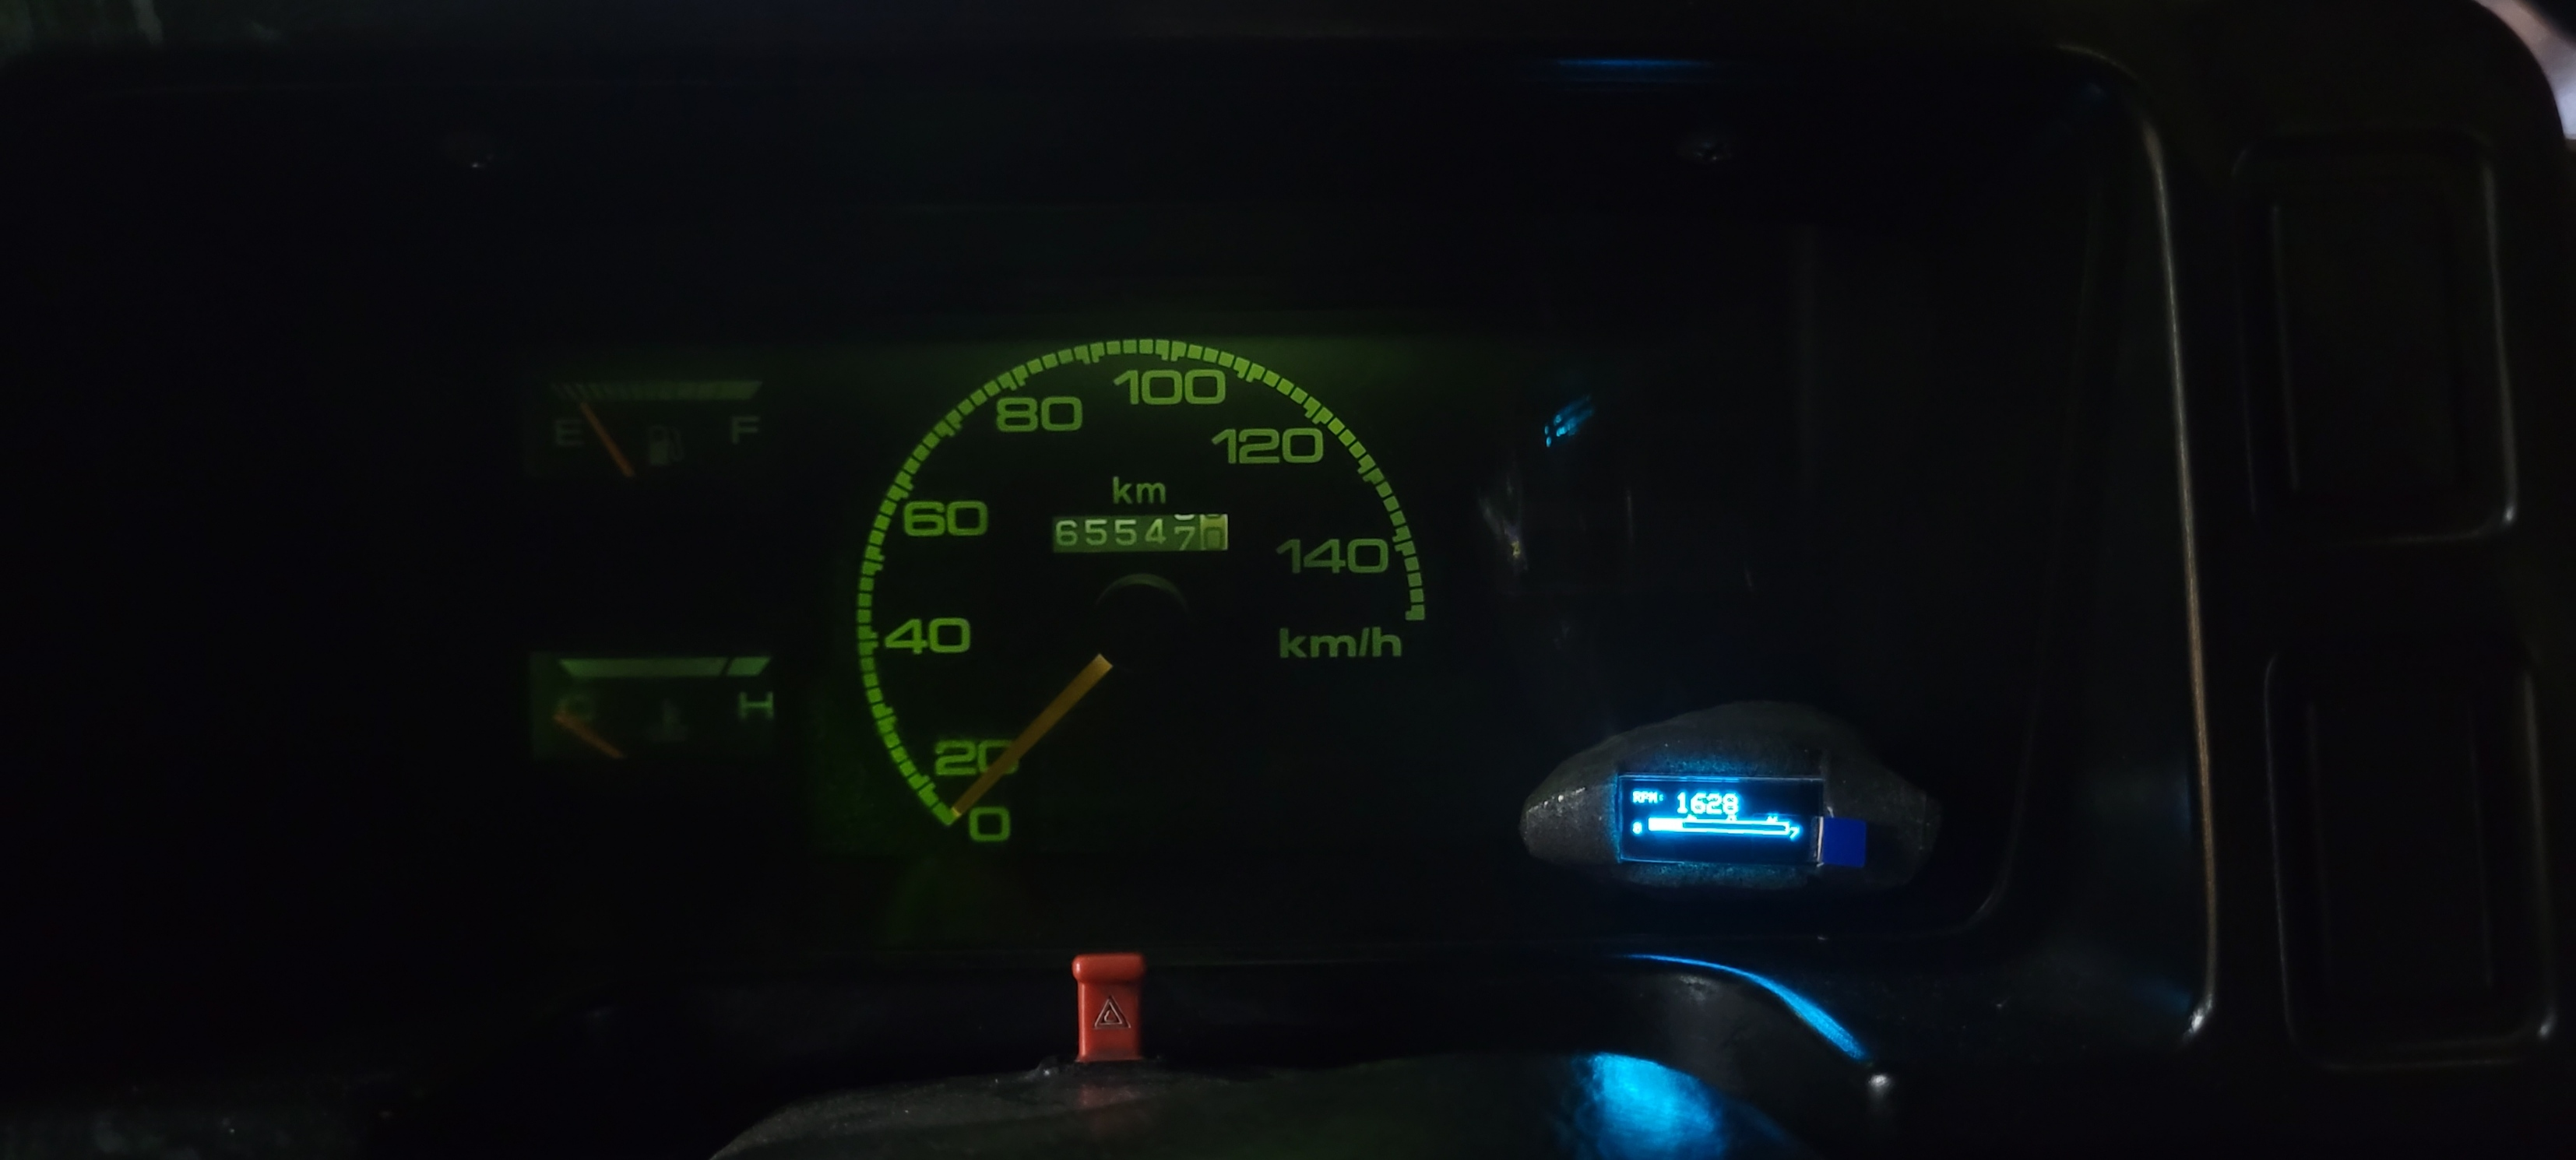
\includegraphics[width=\columnwidth]{dashboard-idle-1.jpg}
\caption{Operational prototype mounted inside the vehicle cluster displaying live idle telemetry.}
\label{fig:dashboard1}
\end{figure}

\begin{figure}[!ht]
\centering
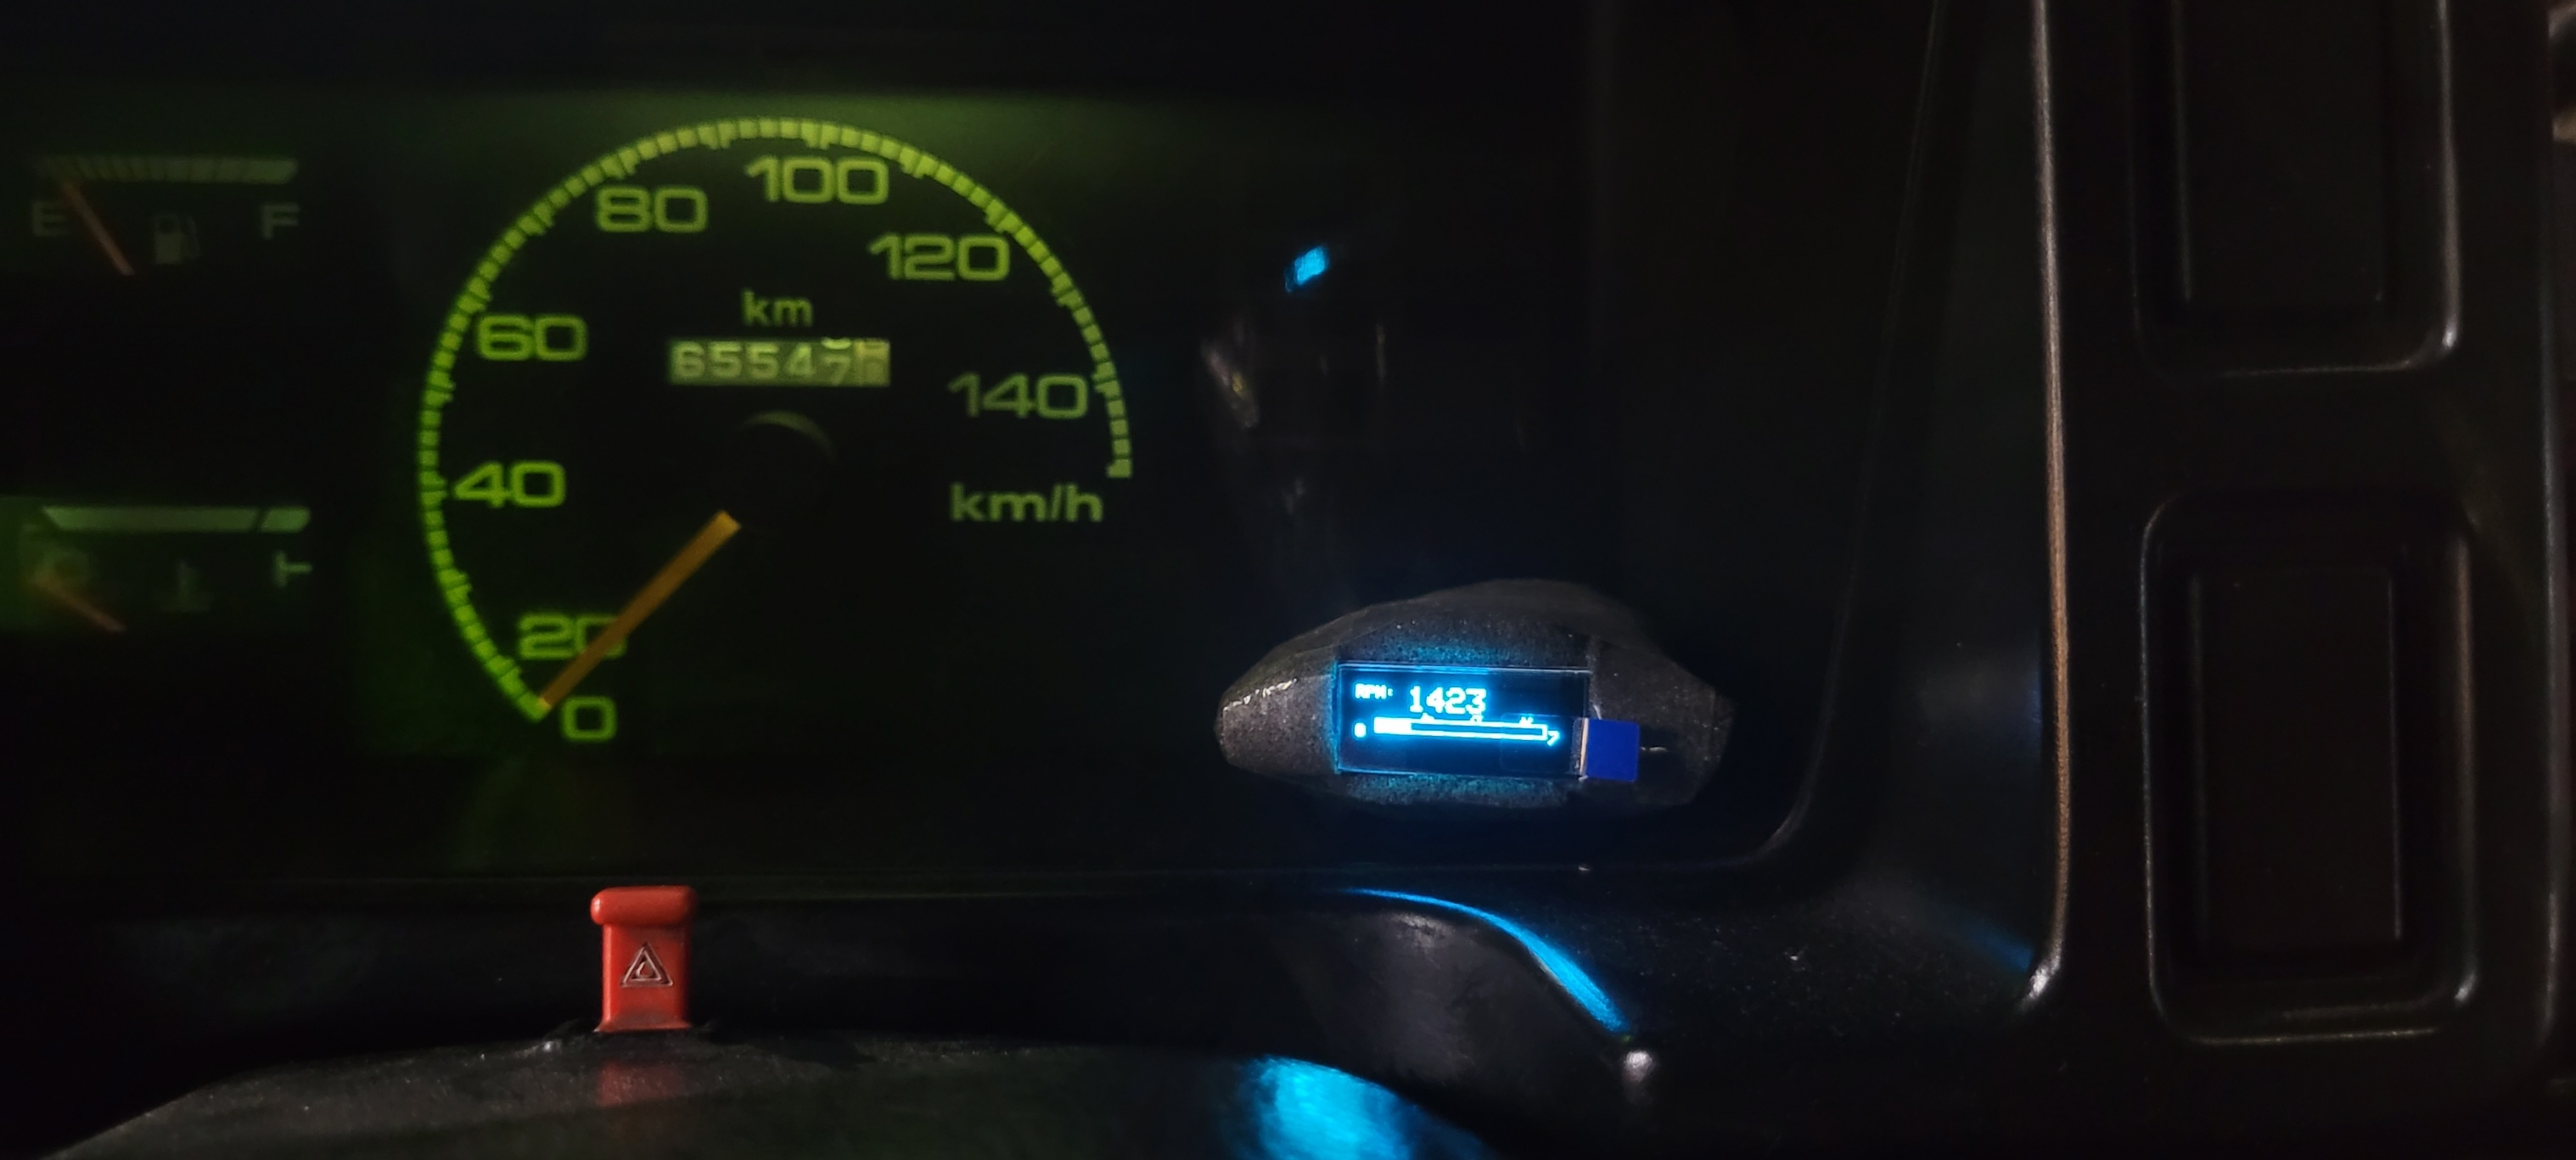
\includegraphics[width=\columnwidth]{dashboard-idle-2.jpg}
\caption{Alternative operational view of the OLED tachometer integrated alongside factory instrument cluster elements.}
\label{fig:dashboard2}
\end{figure}

\subsection{I2C Bus Stability and Electromagnetic Interference}
During periods of sudden high engine load, the OLED display occasionally froze, locking the digital RPM integer and analog bar graph at a fixed value while the engine continued to operate normally. This hardware lockup occurred despite the successful implementation of the aluminum foil shielding on the primary input wire. The anomaly is attributed to intense radiated EMI generated by the ignition coil during wide-open throttle events. While the shielding protected the primary trigger signal, the radiated noise coupled directly into the unshielded I2C data lines (SDA/SCL), corrupting the bus clock state and halting the SSD1306 controller -- a vulnerability distinct from, and not addressed by, the primary-side signal-conditioning techniques of~\cite{signalcond1990,twocycletach1988}, which protect only the ignition-derived trigger signal and not the downstream digital communication bus.

\subsection{Thermal and Power Stability}
The power regulation subsystem demonstrated high resilience to automotive voltage transients. The vehicle's nominal 12--14V rail exhibited severe sag (dropping to 11.2V) during high-current load dumps. The LM2596S buck converter absorbed these fluctuations, maintaining a strictly regulated 7.5V output with negligible thermal dissipation ($\approx 0.3$W).

\section{Discussion}
The transition from a traditional frequency-counting paradigm to an interrupt-driven period measurement successfully resolved the quantization errors typical of low-speed RPM telemetry on legacy three-cylinder architectures, and the error-propagation analysis of Section~III-B quantifies this improvement at roughly four orders of magnitude over the M-method at idle speed. This result is consistent with, and extends to the automotive ignition-pulse domain, the general low-resolution-encoder finding that period (T-method) measurement dominates frequency (M-method) measurement at low speed~\cite{petrella2007,mtmethod2017}. Averaging exactly one complete firing cycle negated the rotational jitter caused by carbureted combustion variance while entirely avoiding the sluggish response times inherent to traditional rolling-average arrays, a result further grounded in the classical coefficient-of-fluctuation-of-speed treatment of flywheel dynamics~\cite{khurmi_tom}. Notably, the same crankshaft-fluctuation signal that this paper's algorithm is designed to reject is, at finer angular resolution and with dedicated crank-angle sensing, the very signal used by OBD-II misfire detectors to identify individual failing cylinders~\cite{rizzoni1989,klenk1993,misfire2011}; a natural extension of the present hardware (discussed below) would exploit this duality.

Field testing highlighted a critical dichotomy in embedded automotive instrumentation: the disparity between analog signal protection and digital bus vulnerability. The integration of the aluminum foil shielding on the input transmission line, combined with the PC817 optocoupler, proved highly effective and is consistent with mitigation strategies described in prior ignition-tachometer signal-conditioning patents~\cite{signalcond1990,twocycletach1988}. However, the system's eventual point of failure under heavy mechanical load was the unshielded I2C bus. Because I2C was originally designed for short-distance, intra-board communication, the jumper wires extending to the dashboard OLED acted as antennas.

To rectify the display freezing without redesigning the physical layout with expensive differential signaling hardware, future iterations of the firmware must implement a software watchdog timer (a ``freeze monitor''). This routine will monitor the display rendering loop; if the I2C bus fails to respond within a specified window, the microcontroller will forcefully reset the I2C bus and reinitialize the SSD1306 controller dynamically. A second avenue for future work, motivated directly by Section~II-C, is to retain the raw (unaveraged) per-pulse period buffer already captured by \texttt{countPulse()} and apply a lightweight per-cylinder uneven-running metric in the style of Klenk \emph{et al.}~\cite{klenk1993} as a secondary diagnostic channel, since the hardware timing infrastructure required is already present and unused between display updates.

\section{Conclusion}
This study establishes a highly optimized, cost-effective framework for retrofitting precision digital telemetry into legacy, mechanically distributed automotive engines. By exploiting hardware-level microsecond timing and exact-cycle integer kinematics -- grounded in the same T-method and M/T-method principles established for low-resolution incremental-encoder speed estimation~\cite{petrella2007,mtmethod2017} -- the proposed tachometer achieves rapid, jitter-free resolution at low engine speeds where commercial frequency-based units fail, a claim substantiated by the closed-form error-propagation analysis of Section~III-B. While the architecture is bound by physical data-starvation during rapid deceleration and is susceptible to severe radiated EMI on unshielded I2C buses, the core methodology provides a rigorous foundation for modernizing classic internal combustion platforms.

\begin{thebibliography}{99}

\bibitem{petrella2007}
R. Petrella, M. Tursini, L. Peretti, and M. Zigliotto, ``Speed measurement algorithms for low-resolution incremental encoder equipped drives: a comparative analysis,'' in \emph{Proc. Int. Aegean Conf. Electrical Machines and Power Electronics (ACEMP)}, 2007.

\bibitem{mtmethod_springer}
``An Improved Variable M/T Method Based on Speed Estimation for Optical Incremental Encoders,'' in \emph{Autonomous and Intelligent Systems}, Lecture Notes in Computer Science, Springer, Berlin, Heidelberg, 2012.

\bibitem{mtmethod2017}
``M/T method based incremental encoder velocity measurement error analysis and self-adaptive error elimination algorithm,'' in \emph{Proc. IECON 2017 -- 43rd Annu. Conf. IEEE Ind. Electron. Soc.}, Beijing, China, 2017.

\bibitem{motioncontroltips}
``How Are Encoders Used for Speed Measurement?'' \emph{Motion Control Tips}, [Online]. Available: https://www.motioncontroltips.com/how-are-encoders-used-for-speed-measurement/

\bibitem{encoderspeedmeasurement}
``Encoder Speed Measurement: Pulse Counting vs. Pulse Timing,'' \emph{Motion Control Tips}, [Online]. Available: https://www.motioncontroltips.com/

\bibitem{indmonitor}
``Calculating Encoder Speed Measurement Accuracy: Period vs. Count Method,'' Industrial Monitor Direct, [Online]. Available: https://industrialmonitordirect.com/blogs/knowledgebase/rotary-speed-measurement-method-1-vs-method-2-accuracy-calculation

\bibitem{motorcontrolpatent}
Y.-J. Kim \emph{et al.}, ``Apparatus and Method of Controlling a Driving Speed of a Motor,'' U.S. Patent 6,819,074, Nov. 16, 2004.

\bibitem{krattenmacher1989}
W. R. Krattenmacher, ``Tachometer, RPM Processor and Method,'' U.S. Patent 4,811,255, Mar. 7, 1989.

\bibitem{nissan1992}
``Tachometer Signal Generating Device,'' U.S. Patent 5,085,191, Feb. 4, 1992.

\bibitem{signalcond1990}
``Tachometer Signal Conditioning Circuit,'' U.S. Patent 4,950,983, Aug. 21, 1990.

\bibitem{twocycletach1988}
``Two and Four Cycle Digital Tachometer,'' U.S. Patent 4,687,991, Aug. 18, 1987.

\bibitem{arduinoforum2023}
``Tachometer Project'' and ``Tachometer from Ignition Coil,'' community engineering discussion threads, Arduino Forum, [Online]. Available: https://forum.arduino.cc/

\bibitem{rizzoni1989}
G. Rizzoni, ``Estimate of Indicated Torque From Crankshaft Speed Fluctuations: A Model for the Dynamics of the IC Engine,'' \emph{IEEE Trans. Veh. Technol.}, vol. 38, no. 3, pp. 168--179, Aug. 1989.

\bibitem{klenk1993}
M. Klenk, W. Moser, W. Mueller, and W. Wimmer, ``Misfire Detection by Evaluating Crankshaft Speed -- A Means to Comply with OBD II,'' SAE Technical Paper 930399, 1993.

\bibitem{misfire2011}
``Engine Misfire Detection Using Crankshaft Speed Multiple Filtering,'' in \emph{Proc. IEEE Int. Conf. on Vehicular Electronics and Safety / related IEEE conference}, 2011.

\bibitem{khurmi_tom}
R. S. Khurmi and J. K. Gupta, \emph{Theory of Machines}, Ch.\ 22: ``Turning Moment Diagrams and Flywheel,'' S. Chand Publishing, New Delhi, India.

\bibitem{lomakin2018}
V. Lomakin, ``Decreasing of Speed Fluctuation of Internal Combustion Engine by Improving the Flywheel Design,'' Ph.D. dissertation, National Transport University, Kyiv, Ukraine, 2018.

\bibitem{lm2596datasheet}
Texas Instruments, ``LM2596 SIMPLE SWITCHER Power Converter 150-kHz 3-A Step-Down Voltage Regulator,'' Datasheet SNVS124G, Nov. 1999, revised Mar. 2023.

\bibitem{pc817datasheet}
``PC817 Series: 1-Channel Transistor Output Type Photocoupler,'' Technical Datasheet, isolation voltage $V_{ISO}=5{,}000\,\text{V}_{rms}$, CTR $\geq 50\%$ at $I_F=5\,\text{mA}$.

\end{thebibliography}

\end{document}